\documentclass[border=2pt]{standalone}
\usepackage{tikz}
\usetikzlibrary{positioning}
\begin{document}
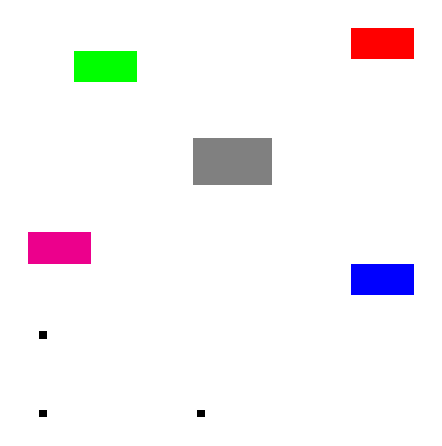
\begin{tikzpicture}[probe/.style={minimum width=8mm,minimum height=4mm,inner sep=0pt,outer sep=0pt}]
  \fill (-.5mm,-.5mm) rectangle (.5mm,.5mm);
  \fill (19.5mm,-.5mm) rectangle (20.5mm,.5mm);
  \fill (-.5mm,9.5mm) rectangle (.5mm,10.5mm);
  \node[fill=gray,minimum width=10mm,minimum height=6mm,inner sep=0pt,outer sep=0pt] (a) at (24mm,32mm) {};
  % No node distance option: the positioning library's default is a pair.
  \node[probe,fill=red,above right=of a] {};
  \node[probe,fill=green,above left=10mm of a] {};
  \node[probe,fill=blue,below right=10mm and 10mm of a] {};
  \node[probe,fill=magenta,below left=6mm and 13mm of a] {};
\end{tikzpicture}
\end{document}
